\chapter{Literature Review}
\section{Introduction}
Engunity AI has emerged as a significant innovation in the field of AI-driven research and development platforms, particularly with the integration of large language models, code automation, and blockchain-backed security. With growing applications in domains such as academic research, software engineering, and data analytics, the demand for intelligent, scalable, and secure AI ecosystems has accelerated the development of platforms like Engunity AI.

Traditional research and coding workflows are often fragmented, requiring users to switch between multiple tools for documentation, computation, and data processing. Recent advancements in AI-assisted systems highlight a shift toward unified SaaS platforms, where models like Groq and Phi-2 enable seamless interaction across research, coding, and data analysis through natural language interfaces. These architectures greatly reduce manual effort, streamline collaboration, and ensure consistent performance through hybrid cloud-local deployment.

Current research and industry efforts are increasingly focused on improving AI reliability, workflow automation, and security integration. This study explores how Engunity AI combines large language models, retrieval-augmented generation (RAG), and blockchain-based provenance to redefine the future of intelligent, secure, and scalable research ecosystems, positioning it as a transformative step in the evolution of AI-powered SaaS infrastructures.



\pagebreak


\section{Overview of the Topic}

Engunity AI represents an advanced AI-powered SaaS platform that unifies research assistance, code generation, and data analysis within a single intelligent ecosystem. The platform is designed to simplify and automate complex workflows that traditionally require multiple disconnected tools and manual effort. By integrating large language models (LLMs), retrieval-augmented generation (RAG), and secure blockchain modules, Engunity AI provides a seamless environment for users to perform research, coding, and data operations efficiently and securely.

The primary objective of the project is to develop a modular, scalable, and cost-efficient architecture that leverages both cloud-based LLMs (Groq) and local fallback models (Phi-2). This hybrid configuration ensures high performance, reduced latency, and resilience even in offline or limited-access environments. Additionally, the system incorporates a FastAPI backend, Next.js frontend, and FAISS-based vector store, enabling intelligent document Q&A, automated research support, and code execution through Docker-based sandboxes.

Engunity AI further distinguishes itself through its blockchain-backed security and provenance features, including decentralized identity verification, smart contract auditing, and on-chain content registration. These elements collectively ensure trust, transparency, and accountability in AI-generated content. The platform’s unified design supports a broad spectrum of applications—from academic research and software development to enterprise analytics—positioning Engunity AI as a pioneering step toward a secure, scalable, and intelligent AI research infrastructure.
\pagebreak


\section{Theoretical Framework}

\begin{figure}[ht]
    \centering
    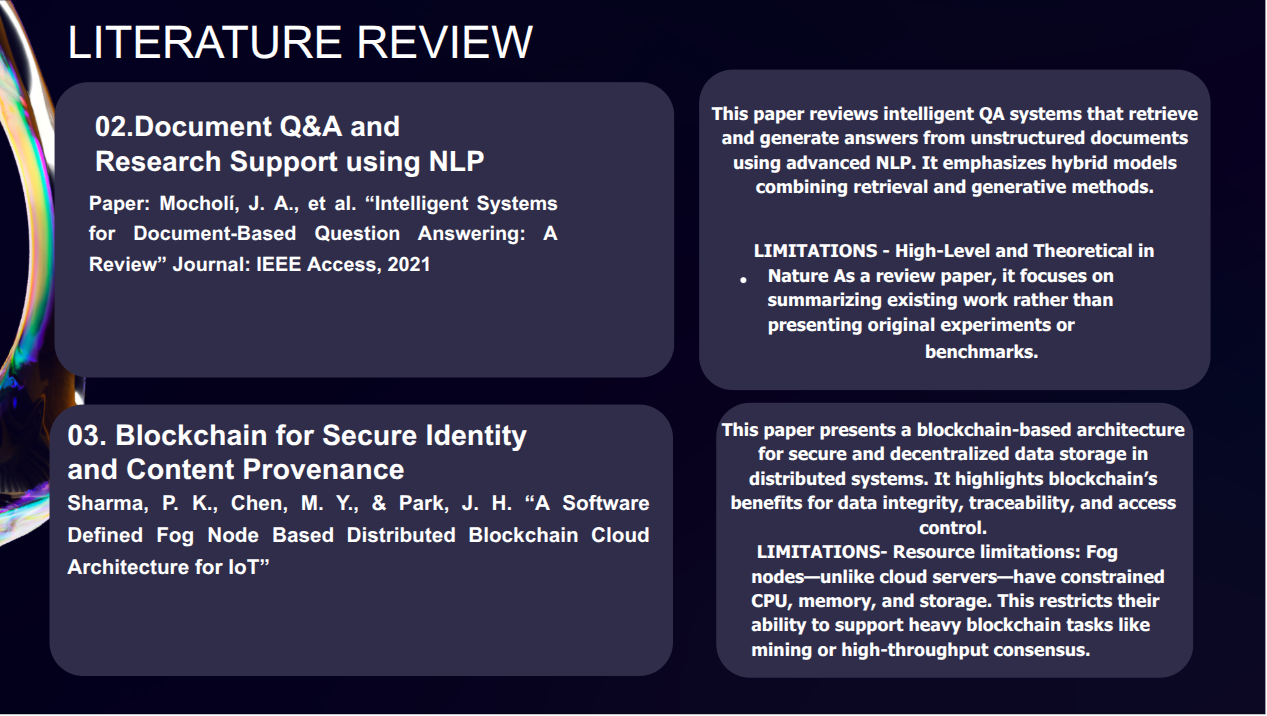
\includegraphics[scale=0.35]{images/Screenshot from 2025-10-08 00-00-53.png}
    
    \label{fig:single}
\end{figure}
\pagebreak


\section{Summary}
Engunity AI builds upon a wide range of advancements in artificial intelligence, cloud computing, and blockchain security. Several foundational studies and frameworks have influenced the system’s architecture, emphasizing scalability, multimodal integration, and secure AI deployment.

Retrieval-Augmented Generation for Knowledge-Intensive NLP Tasks
Authors: Patrick Lewis, Ethan Perez, Aleksandra Piktus, et al.
Published: 2020
Focus: This work introduced the concept of RAG (Retrieval-Augmented Generation), combining retrieval mechanisms with generative models to enhance factual accuracy in AI responses. Engunity AI employs this approach in its Document Q&A module to deliver context-aware, source-grounded answers from uploaded research documents.

Attention Is All You Need
Authors: Ashish Vaswani, Noam Shazeer, Niki Parmar, et al.
Published: 2017
Focus: This paper proposed the Transformer architecture, the foundation for modern large language models (LLMs). Engunity AI leverages transformer-based models (Groq and Phi-2) for natural language understanding, code generation, and intelligent research assistance.

Language Models are Few-Shot Learners (GPT-3)
Authors: Tom B. Brown, Benjamin Mann, Nick Ryder, et al.
Published: 2020
Focus: GPT-3 demonstrated the potential of large-scale pre-trained models to perform multiple downstream tasks with minimal fine-tuning. Engunity AI integrates similar capabilities through its AI Chatbot and Code Assistant modules, enabling flexible adaptation to diverse user inputs.

Blockchain-Based Decentralized Identity and Content Provenance Systems
Authors: Shermin Voshmgir, Trent McConaghy, et al.
Published: 2021
Focus: This research highlights how blockchain technology can ensure transparency, authentication, and traceability in digital systems. Engunity AI applies these principles in its Blockchain Security Layer, ensuring decentralized identity verification, smart contract auditing, and on-chain content registration for AI-generated data.

\pagebreak